\chapter{Learning Single Source Categories}
In this chapter, we study the problem that transfer the knowledge from a single source to recognize single source self-defined categories. As we mentioned in Chapter \ref{sec:intro}, we defined two kinds of self-defined categories: single-source and multi-source self-defined categories. We first introduce our strategy to handle single source categories and the multi-source can be solved using the similar strategy.

To deal with this problem, we firstly propose a data argumentation strategy for single source category. We use the transfer parameters to control the amount of knowledge transferred from the source. To estimate the transfer parameters, we propose a novel objective function that be solved effectively and avoid negative transfer. With extensive experiments on the public benchmark MNIST, we empirically show that our method can effectively transfer the knowledge from a single source and avoid negative transfer while other benchmark transfer methods suffer.

\hl{The rest of this chapter is organized as follow:}
\section{Issues in Transfer Learning}
The motivation of transfer knowledge between different domains is to apply the previous information from the source domain to the target one, assuming that there exists certain relationship, explicit or implicit, between the  feature space of these two domains \cite{pan2010survey}. Technically, previous work can be concluded into solving the following three issues: what, how and when to transfer \cite{tommasi2014learning}.


\textbf{What to transfer.} Previous work tried to answer this question from three different aspects: selecting transferable instances, learning transferable feature representations and transferable model parameters. Instance-based transfer learning assume that part of the instances in the source domain could be re-used to benefit the learning for the target domain. Lim et al. proposed a method of augmenting the training data by borrowing data from other classes for object detection \cite{lim2012transfer}. Learning transferable features means to learn common feature that can alleviate the bias of data distribution in target domain. Recently, Long et al. proposed a method that can learn transferable features with deep neural network and showed some impressive results on the  benchmarks \cite{LongICML15}. Parameter transfer
approach assumes that the parameters of the model for the source task can be transfered to the target task. Yang et al. proposed Adaptive SVMs by transferring parameters by incorporating the auxiliary classifier trained from source domain \cite{yang2007cross}. On top of Yang's work, Ayatar et al. proposed PMT-SVM that can determine the transfer regularizer according to the target data automatically \cite{aytar2011tabula}. Tommasi et al. proposed Multi-KT that can utilize the parameters from multiple source models for the target classes  \cite{tommasi2014learning}.
Kuzborskij et al. proposed a similar method to learn new categories by leveraging over the known source \cite{kuzborskij2013n}.

\textbf{When and how to transfer.} The question \textit{when to transfer} arises when we want to know if the information acquired from previous task is relevant to the new one (i.e. in what situation, knowledge should not be transfered). 
\textit{How to transfer} the prior knowledge effectively should be carefully designed to prevent inefficient and negative transfer. Some previous work consists in using generative probabilistic method \cite{davis2009deep} \cite{wang2014active} \cite{zhou2014multi}.  Bayesian learning methods can predict the target domain by combining the prior source distribution to generate a posterior distribution. Alternatively, some previous max margin methods show that it is possible to learn from a few examples by minimizing the  Leave-One-Out (LOO) error for the training model \cite{kuzborskij2013n} \cite{tommasi2010safety}. Previous work shows that there is a closed-form implementation of LOO cross-validation that can generate unbiased model estimation for LS-SVM \cite{cawley2006leave}.

\hl{Our work correspond to the context above. In this chapter, I propose SMITLe based on parameter transfer approach with LS-SVM. I address my work on how to prevent negative transfer when the source data is not accessible. Compared to other works, I propose a novel strongly convex objective function for transfer parameters estimation. I show that SMITLe can converge at the rate of $O(\frac{\log(t)}{t})$. 
By optimizing this objective function, SMITLe can autonomously adjust the transfer parameters for different prior knowledge. I theoretically and empirically show that, without any data distribution assumption, the superior bound of the training loss for SMITLe is the loss of a method learning directly (i.e. without using any prior knowledge). Experiment results show that when the prior knowledge hurts the transfer procedure, SMITLe can avoid negative transfer by ignoring the unrelated prior knowledge autonomously. Extensive experiments also show that when the prior knowledge is very related (positive transfer), my method can outperform other methods by exploiting the prior knowledge greatly.}

\section{Related Work}\label{sec:single:rl}
In this part, We will introduce the framework my work based on and some related previous work. We first introduce the basic principle of LS-SVM. Based on LS-SVM, several transfer methods are introduced, including A-SVM, PMT-SVM, Multi-KT and MULTIpLe. In these methods, the first two can only adopt the knowledge from single source model and the rest can adopt the knowledge from multiple ones.
\subsection{LS-SVM Classifier}
Least Square SVM is proposed is least squares versions of support vector machines (SVM), which are a set of related supervised learning methods that analyze data and recognize patterns \cite{suykens1999least}. By replacing the hinge loss in classical SVM with L2 loss, LS-SVM classifier is obtained by reformulating the minimization problem as: 
\begin{equation}\label{eq:gama:lssvm}
\begin{aligned}
\min \qquad& L_{LSSVM} = \frac{1}{2}{\left\| w \right\|^2} + \frac{C}{2}\sum\limits_{i = 1}^l {{\varepsilon_i ^2}}\\
\text{s.t.}\qquad&{y_i} = w{x_i} + b + {\varepsilon _i} \quad   \text{for} \quad i \in \left\{ {1,2,...,l} \right\}
\end{aligned}
\end{equation}

The primal Lagrangian for this optimization problem given the unconstrained minimization problem can be written as:
\begin{equation}\label{sq:gama:lsprime}
  L\left( {w,b,\alpha ,\varepsilon } \right) = \frac{1}{2}{\left\| w \right\|^2} + \frac{C}{2}\sum\limits_{i = 1}^l {{\varepsilon _i}^2}  - \sum\limits_{i = 1}^l {{\alpha _i}\left\{ {w{x_i} + b + {\varepsilon _i} - {y_i}} \right\}}
\end{equation}

Where $\alpha = [ \alpha_1,...,\alpha_l]^T $ is the vector of Lagrange multipliers. The solution to minimise this problem is give by:
\begin{equation}
  \left[ {\begin{array}{*{20}{c}}
{K  + \frac{1}{C}{\rm I}}\\
1^T
\end{array}\begin{array}{*{20}{c}}
1\\
0
\end{array}} \right]\left[ {\begin{array}{*{20}{c}}
\alpha \\
b
\end{array}} \right] = \left[ \begin{array}{l}
y\\
0
\end{array} \right]
\end{equation}
Where $K \in R^{l \times l},K_{i,j}=x_i \times x_j^T$. $I$ is the identity matrix and $\mathbf{1}$ is a column vector with all its elements equal to 1. With:
\begin{equation}\label{eq:gama:psi}
\psi^{-1} = \left[ {\begin{array}{*{20}{c}}
{K  + \frac{1}{C}{\rm I}}\\
1^T
\end{array}\begin{array}{*{20}{c}}
1\\
0
\end{array}} \right]^{-1}
\end{equation}
Problem \eqref{sq:gama:lsprime} can be solved by:
\begin{equation}
\left[ {\begin{array}{*{20}{c}}
\alpha \\
b
\end{array}} \right] = \psi^{-1}\left[ \begin{array}{l}
y\\
0
\end{array} \right]
\end{equation}
\subsection{ASVM \& PMT-SVM}
Adaptive SVM (ASVM) is the first work using LS-SVM for transfer learning for vision related tasks \cite{yang2007adapting}. The goal of ASVM is to minimize the distance between the target hyperplane $w$ and source one $w'$ incorporating with the transfer parameter $\gamma$. The objective function is defined as follow:
\begin{equation}\label{eq:gama:asvm}
\begin{aligned}
\min \qquad& L_{ASVM} = \frac{1}{2}{\left\| w - \gamma w' \right\|^2} + \frac{C}{2}\sum\limits_{i = 1}^l {{\varepsilon_i ^2}}\\
\text{s.t.}\qquad&{y_i} = w{x_i} + b + {\varepsilon _i} \quad   \text{for} \quad i \in \left\{ {1,2,...,l} \right\}
\end{aligned}
\end{equation}

Here, $\gamma$ controls the amount of transfer regularization. Intuitively, the regularization term of ASVM is like a spring between $w$ and $\gamma w'$. Equivalently, assume ${\left\| {w'} \right\|^2}=1$ and the regularization term can be expended as:
\begin{equation*}
{\left\| {w - \gamma w'} \right\|^2} = {\left\| w \right\|^2} - 2\gamma \left\| w \right\|\cos \theta  + {\gamma ^2}
\end{equation*}
Where $\theta$ is the angel between $w$ and $w'$. However, the term $-\gamma \left\| w \right\|\cos \theta$ also encourages $||w||$
to be larger (as this reduces the cost) which prevents margin maximization. Thus $\gamma$, which defines the amount of transfer regularization, becomes a tradeoff parameter between margin maximization and knowledge transfer.
\begin{figure}
\centering
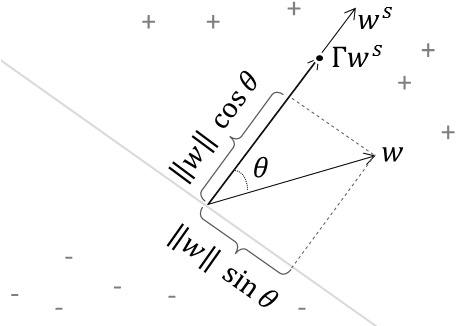
\includegraphics[scale=.6]{transfer/fig/pmt-svm.png}
\caption{Projecting $w$ to $w'$ in PMT-SVM (adapted from \cite{aytar2011tabula}).}\label{fig:gama:pmt}
\end{figure}

Based on this, Projective Model Transfer SVM (PMT-SVM) is proposed to solve the transfer problem by optimizing the following objective function \cite{aytar2011tabula}:
\begin{equation}\label{eq:gama:pmt}
\begin{aligned}
\min \qquad& {L_{PMT}} = \frac{1}{2}{\left\| w \right\|^2} + \gamma {\left\| {Pw'} \right\|^2} + \frac{C}{2}\sum\limits_{i = 1}^l {\varepsilon _i^2} \\
\text{s.t.}\qquad&{y_i} = w{x_i} + b + {\varepsilon _i} \quad   \text{for} \quad i \in \left\{ {1,2,...,l} \right\}\\
& w^Tw' \ge 0
\end{aligned}
\end{equation}

Where $P$ is the the projection matrix $P = I - \frac{{w{'^T} \times w'}}{{w' \times w{'^T}}}$. Therefore, ${\left\| {Pw} \right\|^2} = {\left\| w \right\|^2}{\sin ^2}\theta $ is the
squared norm of the projection of the $w$ onto the source hyperplane (see Figure \ref{fig:gama:pmt}). As $\gamma \rightarrow 0$, the loss function \eqref{eq:gama:pmt} becomes a classic LS-SVM loss function. Because \eqref{eq:gama:pmt} is convex, it can be solved effectively by quadratic optimization.

In summary, both ASVM and PMT-SVM are designed to answer the question: how to transfer by solving some convex objective function. However, they both require a pre-defined parameter $\gamma$, which controls the amount of the knowledge to be transfered, to complete the objective function. In most cases, this parameter can only be set according to the background knowledge. Also, both methods can only adopt the knowledge from single source model which limits the their performance. 
\subsection{Multi-KT}
To learning from many sources, Multi Model Knowledge Transfer (Multi-KT) is proposed to reply on multiple sources by assigning different weight for each of them \cite{tommasi2014learning}. Similar to the objective function \eqref{eq:gama:asvm}, its objective function is defined as follow: 
\begin{equation}\label{eq:gama:multi}
\begin{aligned}
\min \qquad& {L_{Multi - KT}} = \frac{1}{2}{\left\| {w - \sum\limits_k {{\beta _k}} {{w'}_k}} \right\|^2} + \frac{C}{2}\sum\limits_{i = 1}^l {{\zeta _i}\varepsilon _i^2}  \\
\text{s.t.}\qquad&{y_i} = w{x_i} + b + {\varepsilon _i} \quad   \text{for} \quad i \in \left\{ {1,2,...,l} \right\}
\end{aligned}
\end{equation}
Here, $\beta_k$ is the weight assigned for the $k$th source model and $\zeta _i$ is defined as:
\begin{equation*}
{\zeta _i} = \left\{ {\begin{array}{*{20}{c}}
{\frac{N}{{2{N^ + }}}}&{{\text{if }}{y_i} =1}\\
{\frac{N}{{2{N^ - }}}}&{{\text{if }}{y_i} =- 1}
\end{array}} \right.
\end{equation*}
where $N^+$ and $N^-$ are number of positive and negative examples respectively and $N$ is the total number of examples. 

The primal Lagrangian for optimization problem \eqref{eq:gama:multi} can be written as:
\begin{equation}
{L_{Multi - KT}}\left( {w,\beta ,\varepsilon ,\alpha } \right) = \frac{1}{2}{\left\| {w - \sum\limits_k {{\beta _k}} {{w'}_k}} \right\|^2} + \frac{C}{2}\sum\limits_{i = 1}^l {{\zeta _i}\varepsilon _i^2}  + \sum\limits_{i = 1}^l {{\alpha _i}\left[ {w{x_i} + b + {\varepsilon _i} - {y_i}} \right]} 
\end{equation}
So problem \eqref{eq:gama:multi} can be solved once $\beta$ is set.
Different from ASVM and PMT-SVM which require background knowledge to select proper transfer parameter, Multi-KT can estimate the transfer parameter $\beta$ itself by using the closed-form Leave-One-Out (LOO) error. According to \cite{cawley2006leave}, the closed-form LOO error is defined as:
\begin{equation}\label{eq:gama:loo}
{y_{i}} - {\hat y_{i}} = \frac{{{\alpha _{i}}}}{{\psi_{ii}^{ - 1}}}{\qquad\text{for}}\qquad i = 1,...,l
\end{equation}
Here $\psi_{ii}^{-1}$ is its $ith$ diagonal element of $\psi^{-1}$ in \eqref{eq:gama:psi}.

To estimate $\beta$, a loss function, similar to hinge loss, is defined as: 
\begin{equation}\label{eq:gama:multib}
\begin{aligned}
\text{min} \qquad&{\cal L} = \sum\limits_i^l {{\zeta _i}{{\left| {1 - {y_i}{{\hat y}_i}} \right|}_ + }} \\
\text{s.t.} \qquad& \left\| \beta  \right\| \le 1
\end{aligned}
\end{equation}

Here $|x|_+=max(x,0)$. Intuitively, if $\beta$ is properly set, ${y_i}{{\hat y}_i}$ should be positive for each $i$. However, focusing only on the sign of those quantities would result in a non-convex formulation with many local minima. By adding the $|\cdot|_+$ function, formula \eqref{eq:gama:multib} becomes convex and can be solved by gradient descent method.

\subsection{MULTIpLE}
MULticlass Transfer Incremental LEarning (MULTIpLE) focuses on adding a new class to a existing $N$ class source problem while preserving the performance on the old classes \cite{kuzborskij2013n}. To preserving the overall performance of the classifier among $N+1$ classes, MULTIpLE contains two parts: incremental learning for existing $N$ classes and transfer learning for the new class.

For the existing $N$ classes, MULTIpLE uses the similar strategy as ASVM, setting the transfer parameter $\gamma$ to 1. For the new class, it adopts the strategy of Multi-KT, combining knowledge from existing $N$-class models. As a result, the objective function for the hyperplanes in MULTIpLE is defined as:
\begin{equation}
\begin{aligned}
\text{min}\qquad {} & L_{MULTIpLE}=\frac{1}{2}\sum\limits_{n = 1}^N {{{\left\| {{w_n} - {{w'}_n}} \right\|}^2}}  + \frac{1}{2}{\left\| {{w_{N + 1}} - \sum\limits_{k = 1}^N {w{'_k}{\beta _k}} } \right\|^2}+ \frac{C}{2}\sum\limits_{n = 1}^{N + 1} {\sum\limits_{i = 1}^l {\varepsilon _{i,n}^2} }  \\
\text{s.t.}\qquad {} &{\varepsilon _{i,n}} = {Y_{in}} -  {x_i}{w_n} - {b_n}
\end{aligned}\label{eq:gama:multiple}
\end{equation}

Similar like Multi-KT, MULTIpLE uses LOO error in \eqref{eq:gama:loo} to estimate the transfer parameter $\beta$ for the new class. The objective function for $\beta$ estimation is defined by \cite{crammer2002algorithmic}:
\begin{equation}\label{eq:gama:multib}
\begin{aligned}
\text{min} \qquad& {\cal L}\left( {\beta ,i} \right) = \left\{ {\begin{array}{*{20}{c}}
{\mathop {\max }\limits_{n \ne {y_i}} {{\left| {1 - {{\hat Y}_{in}}\left( \beta  \right) - {{\hat Y}_{i{y_i}}}\left( \beta  \right)} \right|}_ + }}&{{:y_i} \ne N + 1}\\
{\left| {1 - {{\hat Y}_{in}}\left( \beta  \right) - {{\hat Y}_{i{y_i}}}\left( \beta  \right)} \right|}&{{:y_i} = N + 1}
\end{array}} \right.  \\
\text{s.t.} \qquad& \left\| \beta  \right\| \le 1
\end{aligned}
\end{equation}
We can find the optimal $\beta$ with projected subgradient descent \cite{BoydCO}. 
\section{Linear Combination Strategy}\label{sec:single:comb}
A major challenge in transferring the knowledge from the source is to design a strategy to combine the source knowledge with the knowledge from the target task. In this section, we propose propose a combination strategy that using linear combination to combine the source and target knowledge. An important advantage of this strategy is that we can adjust the impact of the knowledge comes from the source model more flexibly by just modifying the value of its coefficient. As long as the source knowledge hurts the transfer model, we can reduce its impact to avoid negative transfer.

\hl{Intuitively}, when transferring the knowledge from another task, the performance of the model for the target task is greatly determined by the relationship of these two tasks. Here we use the $\mathcal{H}$-divergence to measure the relationship of two different tasks. $\mathcal{H}$-divergence can be defined as follow:
\begin{definition}
	(from Kifer et al. \cite{kifer2004detecting}) Given a domain $\mathcal{X}$ with two probability distributions, let $\mathcal{H}$ be a hypothesis class on $\mathcal{X}$ and denote by $I(h)$ the set for which $h \in \mathcal{H}$ is the characteristic function where $x\in I(h) \leftrightarrow h(x)=1$. The $\mathcal{H}$-divergence between these two probability distribution $D$ and $D'$ is 
	\begin{equation*}
	{d_{\mathcal{H}}}\left( {D,D'} \right) = 2\mathop {\sup }\limits_{h \in {\mathcal{H}}} \left| {{{\Pr }_D}\left[ {I(h)} \right] - {{\Pr }_{D'}}\left[ {I(h)} \right]} \right|
	\end{equation*}
\end{definition}
When $D$ and $D'$ are related, $d_{\mathcal{H}}\left( {D,D'} \right)$ is small and $d_{\mathcal{H}}\left( {D,D'} \right)$ is large when they are unrelated. Ben et al. \cite{ben2010theory} show that the performance of the target model is affected by the $\mathcal{H}$-divergence of the probability distributions of the two tasks. 

Then our single source self-defined category problem can be described as follow: Given a task  $T$ to distinguish whether an example is from one certain category $C$ from a domain $\mathcal{X} \times \mathcal{Y}$ with $D$ probability distribution over $\mathcal{X}$, $\mathcal{X}$ is the input feature and $\mathcal{Y}$ is the label set $\{1,-1\}$. We use an examples with label 1 to denote the positive example (i.e. belongs to the category) and an example with label -1 to denote the negative example (i.e. not belong to the category). We assume that we have another source model $f'$ trained from another independent task $S$ on another domain $\mathcal{X'} \times \mathcal{Y'}$ with $D'$ probability distribution over $\mathcal{X'}$ and $S$ and $T$ are related. We assume that a small training set $T_{train}=\{(x,y)\} \subset \mathcal{X}\times \mathcal{Y}$, $\mathcal{X}$ is given. We want to learn a classification problem $f: \mathcal{X} \rightarrow \mathcal{X}$ from $T_{train}$ incorporating with $f'$ so that $f$ can perform well on a independent testing set $T_{test}=\{(x,y)\} \subset \mathcal{X} \times \mathcal{Y}$.

Here, let's set the both source and target model $f$ and $f'$ in the hypothesis space of function $\mathcal{H}$ which equals to space of all the linear models of the form. 
\begin{equation}
f(x)=w^Tx+b
\end{equation}
%where $\phi(x)$ is a feature mapping that maps the input space into a another high or even possible infinite dimensional space.

To leverage the knowledge from the source model $f'$, we propose a method where a part of the decision of the target model $f$ comes from the decision of the source model $f'$. This process can be written as:
\begin{equation}\label{eq:single:linear}
\begin{aligned}
 f(x) = & w^T\phi(x)+b+\gamma f'(x) \\
\text{st.} \qquad & f'(x) = w'^T\phi(x)
\end{aligned}
\end{equation}

\begin{figure}
	\centering
	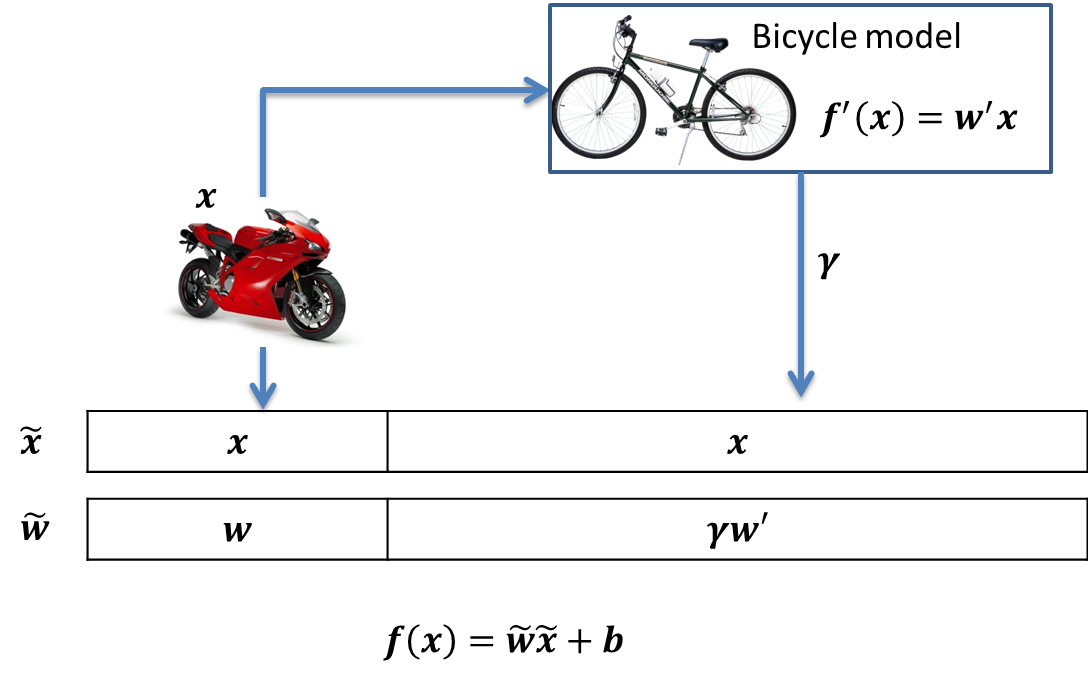
\includegraphics[scale=.6]{transfer/fig/argumentation.png}
	\caption{A graphical representation of linear combination. The score from the source model can be considered as an auxiliary feature and the transfer parameter controls the value of the auxiliary feature.}\label{fig:single:arg}
\end{figure}
Where $\gamma$ is called the transfer parameter $\gamma$ that controls the amount of the knowledge transferred from the source model $f'$. 
While combining the knowledge linearly, we can have several advantages especially when we use linear model such as SVM.

The first advantage is simplicity. Given a example $x$ and a source model $f'$, to consider the decision from the source model, we can simply add its score $f'(x)$ in to affect the decision of the target model. It is equivalent to the data argumentation approach where the score of the source model is used as the auxiliary feature (see Figure \ref{fig:single:arg}). Accordingly, the extra dimension which is set to 1, is added into the hyperplane $w$. By introducing the auxiliary information from the source model, we expect to reduce the bias from the target training set. As a result, we can successfully transfer a transfer learning problem into a traditional machine learning problem with data argumentation.  
Another advantage is flexibility. By using the transfer parameter to control the amount of the knowledge from the source model, the model for the target task is more adaptive to various of situation. Previous work  \cite{kuzborskij2013n} \cite{tommasi2014learning} just consider two situations: unrelated source and positive correlated source. Here we add another situation negative correlated source and expand the previous situation into 3:
\begin{itemize}
	\item When the two tasks are not related, it is expected to get a random score from the source model and the transfer parameter should be set to 0 to ignore it. Therefore, the target model won't affected by the noisy dimension and is less likely to suffer from negative transfer. In the extreme case where the transfer parameter is set 0, no auxiliary information is introduced to the target task and therefore, we can guarantee that, at least, negative transfer won't happen.
	\item When the source and target tasks are positive correlated, i.e. for a positive example $x_p$ and a negative example $x_n$, we have $f'(x_p)>f'(x_n)$, we expect the transfer parameter to be positive. Therefore, the positive and negative examples are more distinct and can be better distinguished by the hyperplane.
	\item  For the same reason above, we expect the transfer parameter to be negative if the two tasks are negative correlated.
\end{itemize}

Therefore, let $\tilde{x} = (x,x)$ and $\tilde{w} = (w,\gamma w')$.
With the LS-SVM setting, our transfer problem can be solved by solving the following optimization problem with argument data:
\begin{equation}\label{eq:single:reg}
	\begin{aligned}
	\min \qquad& L_{LSSVM}(\tilde{w}) = \frac{1}{2}{\left\| \tilde{w} \right\|^2} + \frac{C}{2}\sum\limits_{i = 1}^l {{e_i ^2}}\\
	\text{s.t.}\qquad& \tilde{w} = (w,\gamma w')\\
	&{y_i} = \tilde{w} {\tilde{x_i}} + b + {e _i} \quad   \text{for} \quad i \in \left\{ {1,2,...,l} \right\}\\
	\end{aligned}
\end{equation}
When we consider the transfer parameter $\gamma$ as a constant that can be determined by certain prior knowledge, to regularize  $\left\|\tilde{w}\right\|^2$ is equivalent to regularize $\left\|\tilde{w}-\gamma w'\right\|^2$. Therefore, function \eqref{eq:single:reg} can be represented as:
\begin{equation}\label{eq:single:formreg}
\begin{aligned}
\min \qquad& L_{\gamma}(w) = \frac{1}{2}{\left\| {w}-\gamma w' \right\|^2} + \frac{C}{2}\sum\limits_{i = 1}^l {{e_i ^2}}\\
\text{s.t.}\qquad& {y_i} = {w} {{x_i}} + b + {e _i} \quad   \text{for} \quad i \in \left\{ {1,2,...,l} \right\}\\
\end{aligned}
\end{equation}

To solve the problem \eqref{eq:single:formreg}, we first introduce some important notations used in the rest of this chapter in Table \ref{tab:single:notation}. We use any letter with apostrophe to denote the information from the source data, e.g. if $f(x)$ denotes the model for the target task, $f'(x)$ denotes the model for the source one.

% Table generated by Excel2LaTeX from sheet 'Sheet1'
\begin{table}
	\centering
	\caption{\hl{Notations used in this chapter}}
	\begin{tabular}{|c|L{14cm}|}
		\hline
		$f'(x)$ & binary model for source task \\
		\hline
		$f(x)$  & binary model for target task \\
		\hline
		$\phi(x)$ &  function mapping the input sample into a high dimensional feature space. \\ \hline
		%    $K(x,x)$ & kernel matrix with  $\phi(x_i) \cdot\phi(x_j)$ corresponding to its element $(i,j)$\\ \hline
		$X$     & instance matrix with each row representing one instance \\\hline
		$\boldsymbol{W} $    & (N+1)-column hyperplane matrix for target task. Each column represents one hyperplane of a binary model \\\hline
		$\boldsymbol{W'}$    & hyperplane matrix for the source task \\\hline
		$\boldsymbol{a'} $   & the Lagrangian multiplier matrix for source problem. Each column represents a set of Lagrangian multiplier for a binary SVM model \\\hline
		$\boldsymbol{a} $    & the Lagrangian multiplier matrix for target problem \\
		\hline
		$\boldsymbol{b'},\boldsymbol{b}$  & the bias vector for source and target task \\
		\hline
		$\boldsymbol{a_i}$ & $i_{th}$ column of matrix $\boldsymbol{a}$ \\ \hline
		%    $d_\gamma$ &  diagonal matrix with$\left[ {{\gamma _1},...,{\gamma _N}} \right]$ in its main diagonal\\\hline
		$\boldsymbol{\beta}$ & row vector $\left[ {{\beta _1},...,{\beta _N}} \right]$ to control the prior knowledge for the new category\\ \hline
		$\varepsilon_{ny_i}$&loss parameter. $\varepsilon _{n{y_i}}=1$ if $n=y_i$ and 0 otherwise\\ \hline
		$\psi$, $\psi^{-1}$ & $\psi$ is the modified kernel matrix for solving binary LS-SVM and $\psi^{-1}$ is the inverse matrix of $\psi$\\ \hline
	\end{tabular}%
	\label{tab:single:notation}%
\end{table}%

The primal Lagrangian for this optimization problem \ref{eq:single:formreg} given the unconstrained minimization problem can be written as: 
\begin{equation}
	{L_\gamma }\left( {w,b,\alpha ,e} \right) = \frac{1}{2}{\left\| {w - \gamma w'} \right\|^2} + \frac{C}{2}\sum\limits_{i = 1}^l {{e _i}^2}  - \sum\limits_{i = 1}^l {{\alpha _i}\left\{ {w{x_i} + b + {e_i} - {y_i}} \right\}} 
\end{equation}
The optimal solution can be found by satisfying the following condition:
\begin{eqnarray}\label{eq:single:lssvm-deriv}
\begin{aligned}
\frac{{\partial L}}{{\partial w}} = 0 &\to w = \gamma w' + \sum\limits_i^l {{\alpha _i}{x_i}} \\
\frac{{\partial L}}{{\partial b}} = 0 &\to \sum\limits_i^l {{\alpha _i} = 0} \\
\frac{{\partial L}}{{\partial e_i}} = 0 &\to C{e_i} = {\alpha _i} \qquad i = 1,...,l\\
\frac{{\partial L}}{{\partial {\alpha _i}}} = 0 &\to {y_i} = {w} {{x_i}} + b + {e _i}\qquad i = 1,...,l\\
\end{aligned}
\end{eqnarray}

Let $X=\left[x_1,x_2,...,x_l\right]$ and $Y=[y_1,y_2,...,y_l]$, Eq \eqref{eq:single:lssvm-deriv} can be written in the following compact format:

\begin{equation}\label{eq:single:matrixsolve}
	\left[\begin{array}{cccc}
	\mathbf{I}&0&0&-X^T\\
	0&0&0&-Y^T\\
	0&0&C\mathbf{I}&-I\\
	X&Y&I&0
	\end{array}\right]
	\left[\begin{array}{c}w-\gamma w'\\b\\e\\\alpha
	\end{array}\right]	= \left[\begin{array}{c}0\\0\\0\\\mathbf{1}
	\end{array}\right]
\end{equation} 
where $\mathbf{I}$ is an identity matrix and $\mathbf{1}$ is a column  vector whose elements are 1. 

In real applications, when we have $n$ single source categories and their corresponding source model $f'_1(x),f'_2(x),...,f_n(x)$, their loss function can be represented as:

\begin{equation}\label{eq:single:unionreg}
\begin{aligned}
\min \qquad& L_{\gamma}(w_1,w_2,...,w_n) = \frac{1}{2}\sum\limits_{i = 1}^n{\left\| {w_i}-\gamma_i w_i' \right\|^2} + \frac{C}{2}\sum\limits_{i = 1}^n\sum\limits_{j = 1}^l {{e_{ij} ^2}}\\
\text{s.t.}\qquad& {y_{ij}} = {w_i} {{x_i}} + b_i + {e _{ij}} \quad   \text{for} \quad i \in \left\{ {1,2,...,l}  \right\}, j \in {1,2,...,n}\\
\end{aligned}
\end{equation}
Let $\mathbf{W} = [w_1,w_2,...,w_n]$, $\mathbf{W'} = [w'_1,w'_2,...,w'_n]$ and $D(\gamma)$ be the diagonal matrix $diag(\gamma_1,\gamma_2,...,\gamma_n)$. The corresponding solution for problem \eqref{eq:single:unionreg} is:

\begin{equation}
\left[\begin{array}{cccc}
\mathbf{I}&0&0&-X^T\\
0&0&0&-Y^T\\
0&0&C\mathbf{I}&-I\\
X&Y&I&0
\end{array}\right]
\left[\begin{array}{c}\mathbf{W}- D(\mathbf{\gamma}) \mathbf{W'}\\b\\e\\\alpha
\end{array}\right]	= \left[\begin{array}{c}0\\0\\0\\\mathbf{1}
\end{array}\right]
\end{equation} 
 We can see that Eq. \eqref{eq:single:unionreg} can be solved by directly once the transfer parameters $\gamma=\{\gamma_i|i=1,...,n\}$ is determined.




\section{Cross-Validation Error for LS-SVM}
In this section, we introduce the cross-validation estimation for LS-SVM. As we mentioned in Section \ref{sec:single:comb} that once we determine the value of the transfer parameters $\gamma$, problem \eqref{eq:single:unionreg} can be solved directly. In Section \ref{sec:single:comb}, we treat the transfer parameters as the parameters to be set in advance. In this section, we introduce how we can estimate the unbiased transfer parameters by using an important property of LS-SVM for parameter estimation. 

\subsection{Closed Form Cross-validation Estimation for LS-SVM}
To estimate the transfer parameter, we adopt cross-validation for parameter estimation. Cross-validation is widely used for parameter estimation. Suppose we have a model with one or more unknown parameters, and a data set to which the model can be fit (the dataset). The fitting process optimizes the model parameters to make the model fit the data as well as possible. On the other hand, we have to make sure that this model have the generalization ability, i.e. it can also work well on other independent validation dataset. Otherwise, the model is overfitted to the training data set. However, in practical problem we may not be able to get another independent data set except for the original dataset. Therefore, we have to manually create the validation set by selecting some of the data from the original dataset and use them for evaluation. One round of cross-validation involves partitioning a sample of data into complementary subsets, performing the analysis on one subset (called the training set), and validating the analysis on the other subset (called the validation set or testing set). By repeating these process several rounds with different partitions, we can significant reduce the variability of our estimation using the average results over the rounds.
\begin{figure}
	\centering
	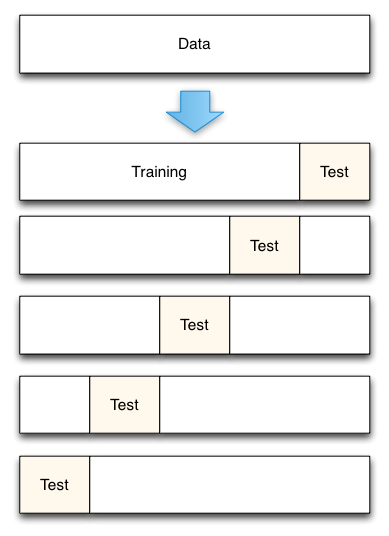
\includegraphics[scale=.4]{transfer/fig/cv.png}
	\caption{An illustration of 5-fold cross-validation}
\end{figure}
There are several different types of cross-validation methods due to their partition strategies. K-fold cross-validation is the most popular type among them. In k-fold cross-validation, the original dataset is randomly partitioned into k equal sized subsamples. K-fold cross-validation is performed in K rounds and in each round, each one of the K partition is used exactly once as the validation set and the rest partitions are used as the training set. 

In our work, we also employ cross-validation for parameter estimation. Here we show that the cross-validation error for LS-SVM can be represented in an efficient way. As a result, we don't have to actually perform cross-validation and re-train the models in each round to obtain the cross-validation error.

\begin{theorem}[An extension of \cite{cawley2006leave}]\label{th:single:cv}
	Given a dataset $D=\{(x_i,y_i)|i=1,...,l\}$, the solution of a LS-SVM on $D$ can be written as Eq. \eqref{eq:gama:lssvm}.
	Assume that $D^{(n)} = \{(x_i,y_i)|i=1,...,n\}$ is a subset of $D$ and $D\backslash D^{(n)}$ is the complement of $D^{(n)}$ in $D$. 
	Let $\left[\alpha_1,...,\alpha_n\right]$ be the corresponding $n$ rows of $\alpha$ in Eq. \eqref{eq:single:orgmatrix} and $S_n$, $s$ and $S_{(l - n + 1)}$ represent the square blocks of matrix:
	
	\begin{equation*}
	\left[ {\begin{array}{c|c}
		{{S_{n }}} &s\\ \hline
		{{s^T}}&{{S_{(l - n + 1)}}}
		\end{array}} \right] =\left[ {\begin{array}{*{20}{c}}
		{K  + \frac{1}{C}{\rm I}}\\
		1^T
		\end{array}\begin{array}{*{20}{c}}
		1\\
		0
		\end{array}} \right]
	\end{equation*}
	The unbiased leave out error of a LS-SVM trained from $D\backslash D^{(n)}$ on $D^{(n)}$ can be estimated as:
	
	\begin{equation*}\label{eq:single:nout}
	ERR_{leave-out} = \left( {{S_n} - sS_{(l - n + 1)}^{ - 1}{s^T}} \right){\left[ {{\alpha _1},...,{\alpha _n}} \right]^T}
	\end{equation*}
\end{theorem}
We show the proof in Appendix \ref{app:cross}. This remarkable result allows cross-validation to be used while only fitting the model once to all available data.

Therefore, we have a convenient solution to estimate the unbiased cross-validation error. However, to perform a cross-validation in practice, decide the partition strategy. Suppose we have $l$ examples in the original data and we want to perform a K-fold cross-validation on it. Thus we have $\mathbf{C^{l/K}_l}$ possible combinations. This means larger K leads to less computation time. Moreover, larger K means less bias towards overestimating the true expected error (as training folds will be closer to the total dataset). When we set $K=l$, we perform $l$-fold cross-validation, i.e. leave-one-out cross-validation (LOO-CV). Vapnik et al. \cite{vapnik2000bounds} show that LOO-CV can provide an almost unbiased estimation error. Previous work also show that transfer learning on the small target training set can be benefit from LOO-CV to better estimate the transfer parameters as well as prevent negative transfer \cite{kuzborskij2013stability}. Due to the reasons above, in this thesis, we use LOO-CV to estimate the transfer parameters to optimize our transfer model.

According to Theorem \ref{th:single:cv}, the LOO-CV error for LS-SVM can be represent as:
\begin{equation}
	ERR_{loo}=\frac{1}{l}\sum_{i}^{l}
\end{equation}